% Four-page short form of the Week 5 QSVM-track report.
%
% Standalone. Same structure, results and numbers as the long form, with the
% extended discussion and three of the six figures dropped.
%
% Build:  latexmk -pdf qsvm_week5_report_short.tex
% Figures: uv run python scripts/make_report_figures.py
%
% Scope: presents results and the limitations OF THOSE RESULTS. Work that was
% never carried out is tracked in NOTES_open_items.md and is absent here.

\documentclass[10pt]{article}

\usepackage[a4paper,margin=0.9in]{geometry}
\usepackage{lmodern}
\usepackage[T1]{fontenc}
\usepackage[utf8]{inputenc}
\usepackage{amsmath,amssymb}
\usepackage{booktabs}
\usepackage{graphicx}
\usepackage{caption}
\usepackage{siunitx}
\usepackage[hidelinks]{hyperref}
\usepackage{microtype}
\usepackage{enumitem}

\captionsetup{font=small,labelfont=bf,skip=4pt}
\sisetup{detect-weight=true,detect-inline-weight=math}
\setlist{nosep,leftmargin=1.2em}
\newcommand{\nc}{\ensuremath{n_{\mathrm{c}}}}
\newcommand{\best}[1]{\textbf{#1}}

\title{\vspace{-2.2em}Isolating the cause of quantum-kernel failure on
malware family attribution\\[0.2em]
\large Short form}
\date{2 August 2026}

\begin{document}
\maketitle
\vspace{-1.8em}

\begin{abstract}
\noindent
A fidelity-kernel quantum SVM (QSVM) falls to the chance level on the 15-class
task of CIC-MalMem-2022 while reaching $0.42$--$0.52$ macro-F1 on the equivalent
EMBER 2018 task, with class imbalance and qubit count already excluded as causes.
We complete the EMBER classical baseline with four models, validate the 1000-row
subsample all quantum results rest on, measure class separability of the shared
PCA projection, and measure kernel concentration and alignment against an RBF
control built on the identical feature matrix. Random forest beats SVM on every
EMBER binary configuration, so the recorded classical advantage was understated
by $0.011$ to $0.027$ macro-F1. All 84 comparable pairs favour the classical
model at $p<0.05$. The RBF control produces the same off-diagonal Gram spread on
both corpora ($0.2212$ against $0.2184$), whereas the fidelity kernel matches RBF
on EMBER ($0.92\times$) and collapses to $0.40\times$ on CIC. The collapse is a
property of the kernel, not of the corpus.
\end{abstract}

\section{Introduction}

Three questions were open. The EMBER classical arm used a support vector machine
only, so every recorded margin there compared against one baseline rather than
the strongest available. The QSVM's collapse on CIC 15-class was unexplained.
And every claim of a classical advantage rested on differences in mean macro-F1
with no test that a gap exceeded fold-to-fold noise. A fourth issue was that all
quantum results are computed on a 1000-row subsample whose fidelity to its
population had been assumed rather than measured.

\section{Materials and methods}

\textbf{Data.} \emph{CIC-MalMem-2022}: memory dumps, 55 forensic features;
\num{58596} balanced rows for the binary task and \num{29298} malware-only rows
over 15 families ($1.7\times$ imbalanced) for the 15-class task.
\emph{EMBER 2018}: static PE features, 2381 dimensions, on an \num{18014}-row
extract of the published test set ($88.9\%$ malware); its 15-class task keeps the
15 largest families and downsamples each to the smallest, giving \num{14325} rows
at 955 per family.

\textbf{Protocol.} Both frameworks consume one pipeline: variance filter,
correlation filter at $0.95$, standardisation, PCA to \nc{} components, fit on
training-fold rows only. \nc{} abbreviates $n_{\mathrm{components}}$ and sets the
classical feature count and the quantum qubit budget simultaneously. The fidelity
kernel costs one circuit evaluation per training pair, so quantum runs use a
stratified 1000-row subsample; that subsample and its five outer folds are
persisted by the quantum runner and replayed by the classical one, giving 800
training and 200 held-out rows per fold.

\textbf{Metric.} Held-out macro-F1 averaged over five folds. Accuracy is not
reported: on EMBER binary at $\nc{}=1$ the QSVM reaches $0.890$ accuracy in three
of five folds while the benign class's F1 is exactly $0.000$, because $88.9\%$ of
rows are malware and the model labels everything malware.

\textbf{Measurements introduced here.} Four classical models at
$\nc{}\in\{1,3,6\}$ on both EMBER tasks; per-feature Kolmogorov--Smirnov tests of
the subsample against its population; Fisher ratio and silhouette of the shared
projection; off-diagonal Gram spread and kernel-target alignment for the fidelity
kernel and for an RBF control on the identical matrix; paired $t$-test and
Wilcoxon over per-fold macro-F1.

\textbf{Run selection.} Fold records are grouped by cross-validation sweep, not by
configuration. The same configuration was swept more than once, so a
parameter-based grouping returns 10, 15 or 20 records for a five-fold sweep, and
for the QSVM the encoding is a per-fold tuner outcome rather than a configuration
key. Only sweeps completing with exactly five folds are retained: 123 of 125.

\section{Results}

\subsection{The classical baseline was incomplete}

\begin{table}[htbp]
\centering
\small
\caption{EMBER 2018 held-out macro-F1, mean over five outer folds. Best classical
model in bold.}
\begin{tabular}{@{}l S[table-format=1.4] S[table-format=1.4] S[table-format=1.4]
S[table-format=1.4] S[table-format=1.4] S[table-format=1.4]@{}}
\toprule
& {Random forest} & {XGBoost} & {LightGBM} & {SVM} & {QSVM angle} & {QSVM IQP} \\
\midrule
\multicolumn{7}{@{}l}{\emph{Binary}}\\
$\nc{}=1$ & \best{0.5582} & 0.5451 & 0.5093 & 0.5314 & 0.4532 & 0.4587 \\
$\nc{}=3$ & \best{0.6575} & 0.6465 & 0.6434 & 0.6306 & 0.4924 & 0.5084 \\
$\nc{}=6$ & \best{0.6835} & 0.6680 & 0.6593 & 0.6724 & 0.5138 & 0.5137 \\
\addlinespace
\multicolumn{7}{@{}l}{\emph{15-class}}\\
$\nc{}=1$ & \best{0.5562} & 0.5313 & 0.5410 & 0.5294 & 0.1688 & 0.1541 \\
$\nc{}=3$ & 0.7194 & 0.7089 & 0.7035 & \best{0.7389} & 0.3908 & 0.4797 \\
$\nc{}=6$ & 0.7903 & 0.7659 & 0.7709 & \best{0.7930} & 0.4232 & 0.5195 \\
\bottomrule
\end{tabular}
\end{table}

Random forest beats SVM on every binary configuration, widening the classical
advantage from $+0.0727$ to $+0.0995$ at $\nc{}=1$, from $+0.1222$ to $+0.1491$
at $3$, and from $+0.1587$ to $+0.1697$ at $6$. On 15-class SVM is the strongest
baseline at $\nc{}\in\{3,6\}$, so those margins stand. Four of six configurations
move, all in the same direction.

\begin{figure}[htbp]
\centering
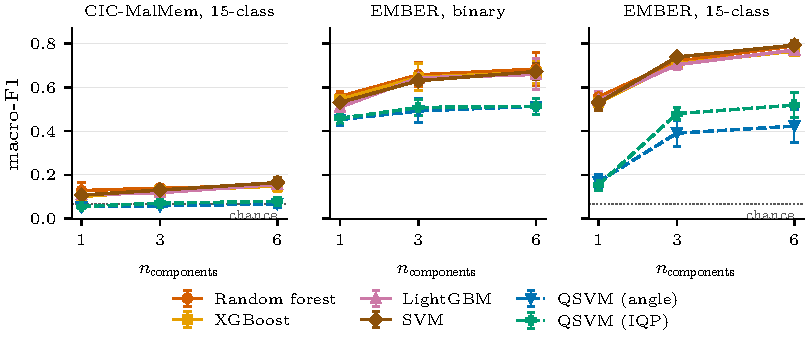
\includegraphics[width=\textwidth]{figures/fig_capacity_scaling.pdf}
\caption{Macro-F1 against the shared feature and qubit budget; solid lines
classical, dashed the QSVM encodings, dotted the 15-class chance level. On EMBER
binary the QSVM gains $0.055$ macro-F1 from one to six components where the
random forest gains $0.125$, so the gap widens with capacity. CIC binary is not
shown, for the reason in §\ref{sec:limits}.}
\end{figure}

\subsection{The subsample preserves its population}

A rejection count is interpretable only against its null expectation, since a
faithful subsample still rejects about $\alpha\cdot n_{\mathrm{features}}$
features by chance. CIC rejects \textbf{0} of 55 where $\approx 2.75$ were
expected, EMBER \textbf{1} of 2381 where $\approx 119$ were. Maximum
class-proportion drift is below $0.001$ on both.

\subsection{Feature geometry accounts for the corpus, not the kernel}

EMBER's families are $\approx 8\times$ more separable by Fisher ratio and up to
$50\times$ on the worst-case family. CIC's silhouette is negative at every \nc{},
so the average point lies closer to another family's centroid than its own. CIC's
PCA nonetheless explains more variance ($33$--$81\%$ against $8$--$30\%$), placing
its variance in directions that do not discriminate family.

This accounts for the poor absolute performance of every method on CIC 15-class.
It does not account for a QSVM-specific deficit, since a classical SVM extracts
$0.108$--$0.165$ macro-F1 from these same features where the QSVM extracts
$0.056$--$0.079$.

\subsection{Kernel concentration accounts for the kernel}
\label{sec:kernel}

\begin{figure}[htbp]
\centering
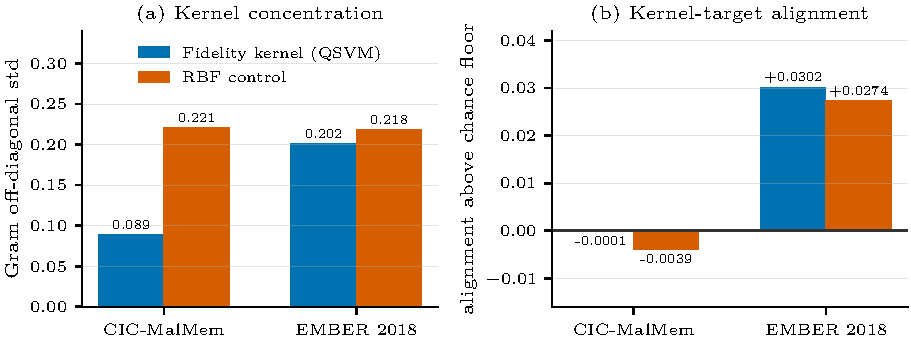
\includegraphics[width=\textwidth]{figures/fig_kernel_diagnostics.pdf}
\caption{First outer training fold, $\nc{}=6$, IQP encoding, 800 rows, with an RBF
control on the identical feature matrix. (a) Off-diagonal Gram spread.
(b) Alignment relative to its floor, a constant kernel scoring
$1/\sqrt{15}\approx 0.258$ on 15 balanced classes.}
\end{figure}

The RBF control produces near-identical spread on both corpora, so CIC's features
do not cause a classical kernel to concentrate. The fidelity kernel tracks RBF on
EMBER at $0.92\times$ and collapses to $0.40\times$ on CIC, compressing every
off-diagonal similarity into a band $2.5\times$ narrower from the same inputs.

On alignment the CIC fidelity kernel lands $0.000069$ \emph{below} the
constant-kernel floor, indistinguishable from a matrix of ones, and the RBF
control is also below it; on EMBER both clear it by $\approx 0.03$. Alignment
separates the corpora while concentration separates the kernels. Across the full
sweep EMBER's Gram is $1.9$--$2.6\times$ more spread than CIC's at every
comparable cell.

\subsection{The differences are statistically significant}

\begin{figure}[htbp]
\centering
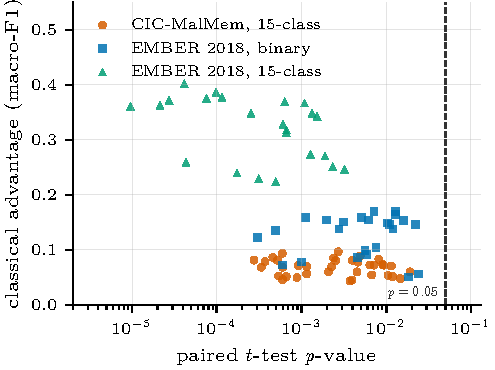
\includegraphics[width=0.50\textwidth]{figures/fig_significance.pdf}
\caption{All 84 comparable quantum--classical pairs. Every point lies left of
$p=0.05$ and above zero.}
\end{figure}

All 84 comparable pairs favour the classical model at $p<0.05$; the largest
$p$-value is $0.0241$. Wilcoxon returns exactly $0.0625$ for all 84, which at five
paired samples is the smallest attainable two-sided value, so the test cannot
reach $0.05$ at this fold count regardless of effect size. Among classical models
on shared predictions, McNemar separates random forest from XGBoost on EMBER
15-class at $p=0.0022$, while on CIC 15-class no classical pair separates at all.

\section{Discussion}

Feature geometry and kernel geometry give different answers, and that difference
is the diagnosis. Geometry explains why every method performs poorly on CIC
15-class but cannot explain a QSVM-specific deficit, since the classical SVM
recovers two to three times the QSVM's macro-F1 from the same projection. Kernel
concentration does explain it: the fidelity kernel loses $60\%$ of the RBF
control's off-diagonal spread on inputs where the control loses none. A Gram
approaching a scaled identity presents the SVM with a geometry in which all pairs
are equally similar, which is what a macro-F1 pinned to chance looks like
internally. The result is a statement about the method rather than the corpus.

\subsection{Limitations}
\label{sec:limits}

\begin{itemize}
\item \textbf{Bandwidth is untested on CIC.} Concentration is the identified
mechanism and bandwidth is the parameter that acts on it, but no sweep was run.
§\ref{sec:kernel} identifies a mechanism, not a remedy.
\item \textbf{Alignment is a weak predictor.} It reports that neither kernel
carries label information on CIC, yet a classical SVM reaches $0.16$ there.
Alignment is a global unweighted average over all pairs and an SVM requires no
such property, so it ranks corpus difficulty usefully and predicts attainable
performance poorly.
\item \textbf{Scope of the kernel measurement.} The alignment and RBF-control
figures come from one training fold, one capacity and one encoding, with a single
untuned $\gamma$ for the control.
\item \textbf{One configuration is not separable.} Every CIC binary run,
classical and quantum alike, predates sweep-level tracking and carries no
recoverable boundary; 45 fold records per model resolve into two sweeps per \nc{}
with no identifier separating them. No grouping was reconstructed. The limitation
is symmetric across frameworks.
\item \textbf{No sample-level test between frameworks.} McNemar needs per-sample
predictions from both models; QSVM predictions were not persisted for these
sweeps, so cross-framework evidence rests on five paired fold-level scores.
\item \textbf{Fold count.} Five folds support the paired $t$-test and are too few
for Wilcoxon. Six would place $0.03125$ within reach.
\item \textbf{Simulator only.} No hardware execution and no noise model.
\end{itemize}

\section{Conclusion}

Completing the classical baseline widened the recorded classical advantage on
EMBER binary by $0.011$ to $0.027$ macro-F1, and paired testing establishes that
all 84 comparable differences reach $p<0.05$. The subsample every quantum result
depends on is faithful to its population. The QSVM's collapse on CIC 15-class is
attributable to kernel concentration rather than to feature difficulty: an RBF
kernel on the identical matrix retains its spread while the fidelity kernel falls
to $0.40\times$ of it, which locates the failure in the kernel and names the
parameter that acts on it.

\end{document}
